\documentclass[10pt]{exam}
\usepackage[phy]{template-for-exam}
\usepackage{tikz,graphicx}

\title{Projectiles \#2}
\author{Rohrbach}
\date{\today}

\begin{document}
\maketitle

\begin{questions}

\question
  A swallow is carrying a coconut horizontally across the ground with an air speed velocity of 11 m/s.  Suddenly, the bird loses his grip on the husk, and it falls to the ground.  The bird is flying at an altitude of 45~meters.

  \begin{parts}
    \part
      \emph{Label} diagram of the situation, and write down knowns and unknowns.
      
      \vspace{2em} 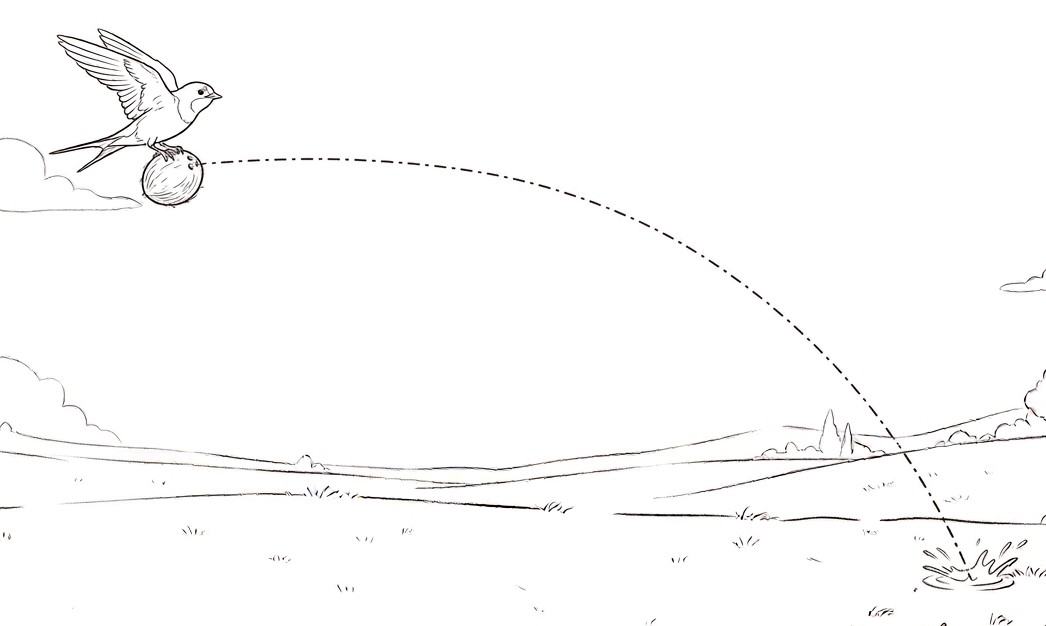
\includegraphics[height=1.5in]{swallow.jpg} \vspace{2em}

    \part
      How much time did it take the coconut to hit the ground?
      \vs
  
    \part
      How far across the ground did the coconut travel?
      \vs
  
    \part
      What is the $x$- and $y$- velocity of the coconut just before hitting the ground?
      \vs
  
    \part
      What is the magnitude and direction of the resultant velocity just before hitting the ground?
      \vs

  \end{parts}

\pagebreak

\question
  A plane is flying 30 m above the ground.  A package is dropped from the plane and travels 50 m horizontally before finally striking the ground.  
  
  \begin{parts}
    \part
      \emph{Label} diagram of the situation, and write down knowns and unknowns.
      
      \vspace{1em}
      %
      \begin{tikzpicture}

        \begin{scope}[shift={(0,3)}]
          \node at (-0.2,.75) {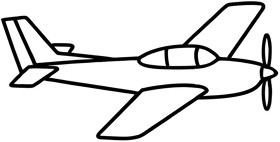
\includegraphics[height=1cm]{airplane}};
          \draw[rounded corners=3px,rotate=10] (0,0) rectangle (0.4,0.4);
        \end{scope}
        

        \begin{scope}[shift={(5,0)}]
          \draw[rounded corners=3px,rotate=10] (0,0) rectangle (0.4,0.4);
        \end{scope}

        \draw[dashed] (0.5,3.3) parabola (5.1,0.37);

        \draw (-2,0) -- (8,0);
      \end{tikzpicture}
      %
      \vspace{2em}
    
    \part
      How long did it take the package to hit the ground?
      \vs
    
    \part
      How fast must the plane have been flying?
      \vs
    
    \part
      What is the $x$- and $y$- velocity of the package just before it hits the ground?
      \vs
    
    \part
      What is the magnitude and direction of the final resultant velocity of the package just before it hits the ground?
      \vs

  \end{parts} 
\end{questions}






\end{document}